\documentclass[a4paper, 14pt, titlepage, fleqn]{extarticle}
\usepackage{cmap}
\usepackage[colorlinks=true, urlcolor=blue, linkcolor=black]{hyperref}
\usepackage[T2A]{fontenc}
\usepackage[utf8]{inputenc}
\usepackage[russian]{babel}
\usepackage{amsmath}
\usepackage{graphicx}
\usepackage{listings}
\usepackage{xcolor}
\usepackage{cases}
\usepackage{float}
\usepackage{url}

\usepackage[]{minted}
\usepackage{tcolorbox}
\usepackage{etoolbox}
\BeforeBeginEnvironment{minted}{\begin{tcolorbox}}%
\AfterEndEnvironment{minted}{\end{tcolorbox}}%

\textwidth 16cm
\textheight 26cm
\oddsidemargin -2.5mm
\evensidemargin -3mm
\topmargin -20mm
\parindent 1.25cm

\definecolor{backcolour}{RGB}{234, 234, 234}
\definecolor{codegreen}{RGB}{9, 130, 0}
\definecolor{codegray}{rgb}{0.5, 0.5, 0.5}
\definecolor{bg}{rgb}{0.15,0.95,0.25}

\usemintedstyle[Python]{xcode}
\newminted{pycon}{bgcolor=bg, linenos=true, tabsize=4}

\begin{document}
	\title{\textbf{Прием и обработка APT сигнала со спутников дистанционного зондирования Земли}}
	\author{Тимофеев Андрей \\ Лебедев Михаил \\ Капцевич Ольга}
	\maketitle
	
	\tableofcontents
	\pagebreak

	\section*{Введние}
	\addcontentsline{toc}{section}{Введние}
	
	Суть проекта заключается в создании станции (на основе RTL-SDR) по приему и обработки \href{https://en.wikipedia.org/wiki/Automatic_picture_transmission}{APT (Automatic Picture Transmission)} сигнала со спутников дистанционного зондирования Земли на базе лаборатории спутниковго мониторинга ДВФУ. \\
	
	\noindent Станция предствляет собой Антену SDR ....
	
	\subsection*{Лаборатория спутниковго мониторинга ДВФУ}
	\addcontentsline{toc}{subsection}{Лаборатория спутниковго мониторинга ДВФУ}
	
	\subsection*{APT (Automatic Picture Transmission)}
	\addcontentsline{toc}{subsection}{APT (Automatic Picture Transmission)}
	
	\textbf{Automatic Picture Transmission} - это стандарт для аналоговой передачи данных (изображений) по радиоканалу с использованием специализированных радиопередатчиков, установленных на метеорологических спутниках. \\ 
	
	\noindent Стандарт APT был разработан подразделением \href{https://www.noaa.gov/}{NOAA National Earth Satellite Service} в 1960-х. Впервые был описан в статье \href{https://ntrs.nasa.gov/api/citations/19630013799/downloads/19630013799.pdf}{``The Automatic Picture Transmission (APT) TV camera system for meteorological satellites''}. Первый спутник на полярной орбите, передававший изображения в формате APT — TIROS-N.
	
	\subsection*{RTL-SDR}
	\addcontentsline{toc}{subsection}{RTL-SDR}
	
	
	
	\pagebreak
	\section*{Аппаратная реализация}
	\addcontentsline{toc}{section}{Аппаратная реализация}
	
	% Аппаратная часть станции представляет собой две антенны
	Для приёма сингала используются две антенны X-Quad на ??? и ??? МГц закреплённые на поворотном устройстве (TODO) на крыше корпуса G кампуса ДВФУ. Поворотное устройство управляется программно с компьютера, находящегося в кабинете G542 (на крышу протянуты провода).
	
	TODO картинки антенн и контрллера поворота
	
	В рамках проекта стояла задача разработать аппаратную систему, позволяющую принимать и обрабатывать радиосигналы с помощью программно определяемых радиосистем (RTL-SDR). Желаемые качества такой системы были следующие:
	\begin{itemize}
		\item \textbf{Возможность непрерывной работы.} Предполагается постоянное функционирование системы.
		\item \textbf{Возможность полной автоматизации.} Предполагается использование станции полностью в автоматическом режиме, включая поворот антенны, начало и конец записи.
		\item \textbf{Отказоустойчивость и простота починки.} Система должна быть достаточно простой, а также простой в ремонте при поломке.
		\item \textbf{Возможность дополнения и обновления.} В данный момент используются модули RTL-SDR, но впоследствии желательна возможность заменить их радиосистемами лучшего качества.
		\item \textbf{Низкая шумность.} Желательно избегать длинных линий передачи слабого аналогового сигнала от антенны к радиоприёмнику.
	\end{itemize}
	
	Руководствуясь этими критериями были разработаны 3 возможные архитектуры системы.
	
	\subsection*{Варианты архитектуры системы}
	\addcontentsline{toc}{subsection}{Варианты архитектуры системы}
	
	В каждом из вариантов архитектуры предполагается расположение части оборудования непосредственно на вращающейся части поворотного комплекса антенн в влагозащищённом контейнере. На схемах ниже эта часть представлена слева и схематически отделена от оборудования в помещении двумя косыми чертами.
	
	Также в каждом из вариантов предполагается питание этого оборудования от источника постоянного тока расположенного в помещении. Для того, чтобы доставить стабильную мощность оборудованию, по линии питания подаётся напряжение 14В и используется регулятор для понижения напряжения до 5В.
	
	\pagebreak
	\subsubsection*{Вариант №1}
	\addcontentsline{toc}{subsubsection}{Вариант №1}
	
	Наиболее предпочтительным вариантом представлялось использование удлинителя USB для подключения RTL-SDR через длинную цифровую линию непосредственно к компьютеру в помещении, на котором развёрнута программная часть системы.
	
	\begin{figure}[H]
		\centering
		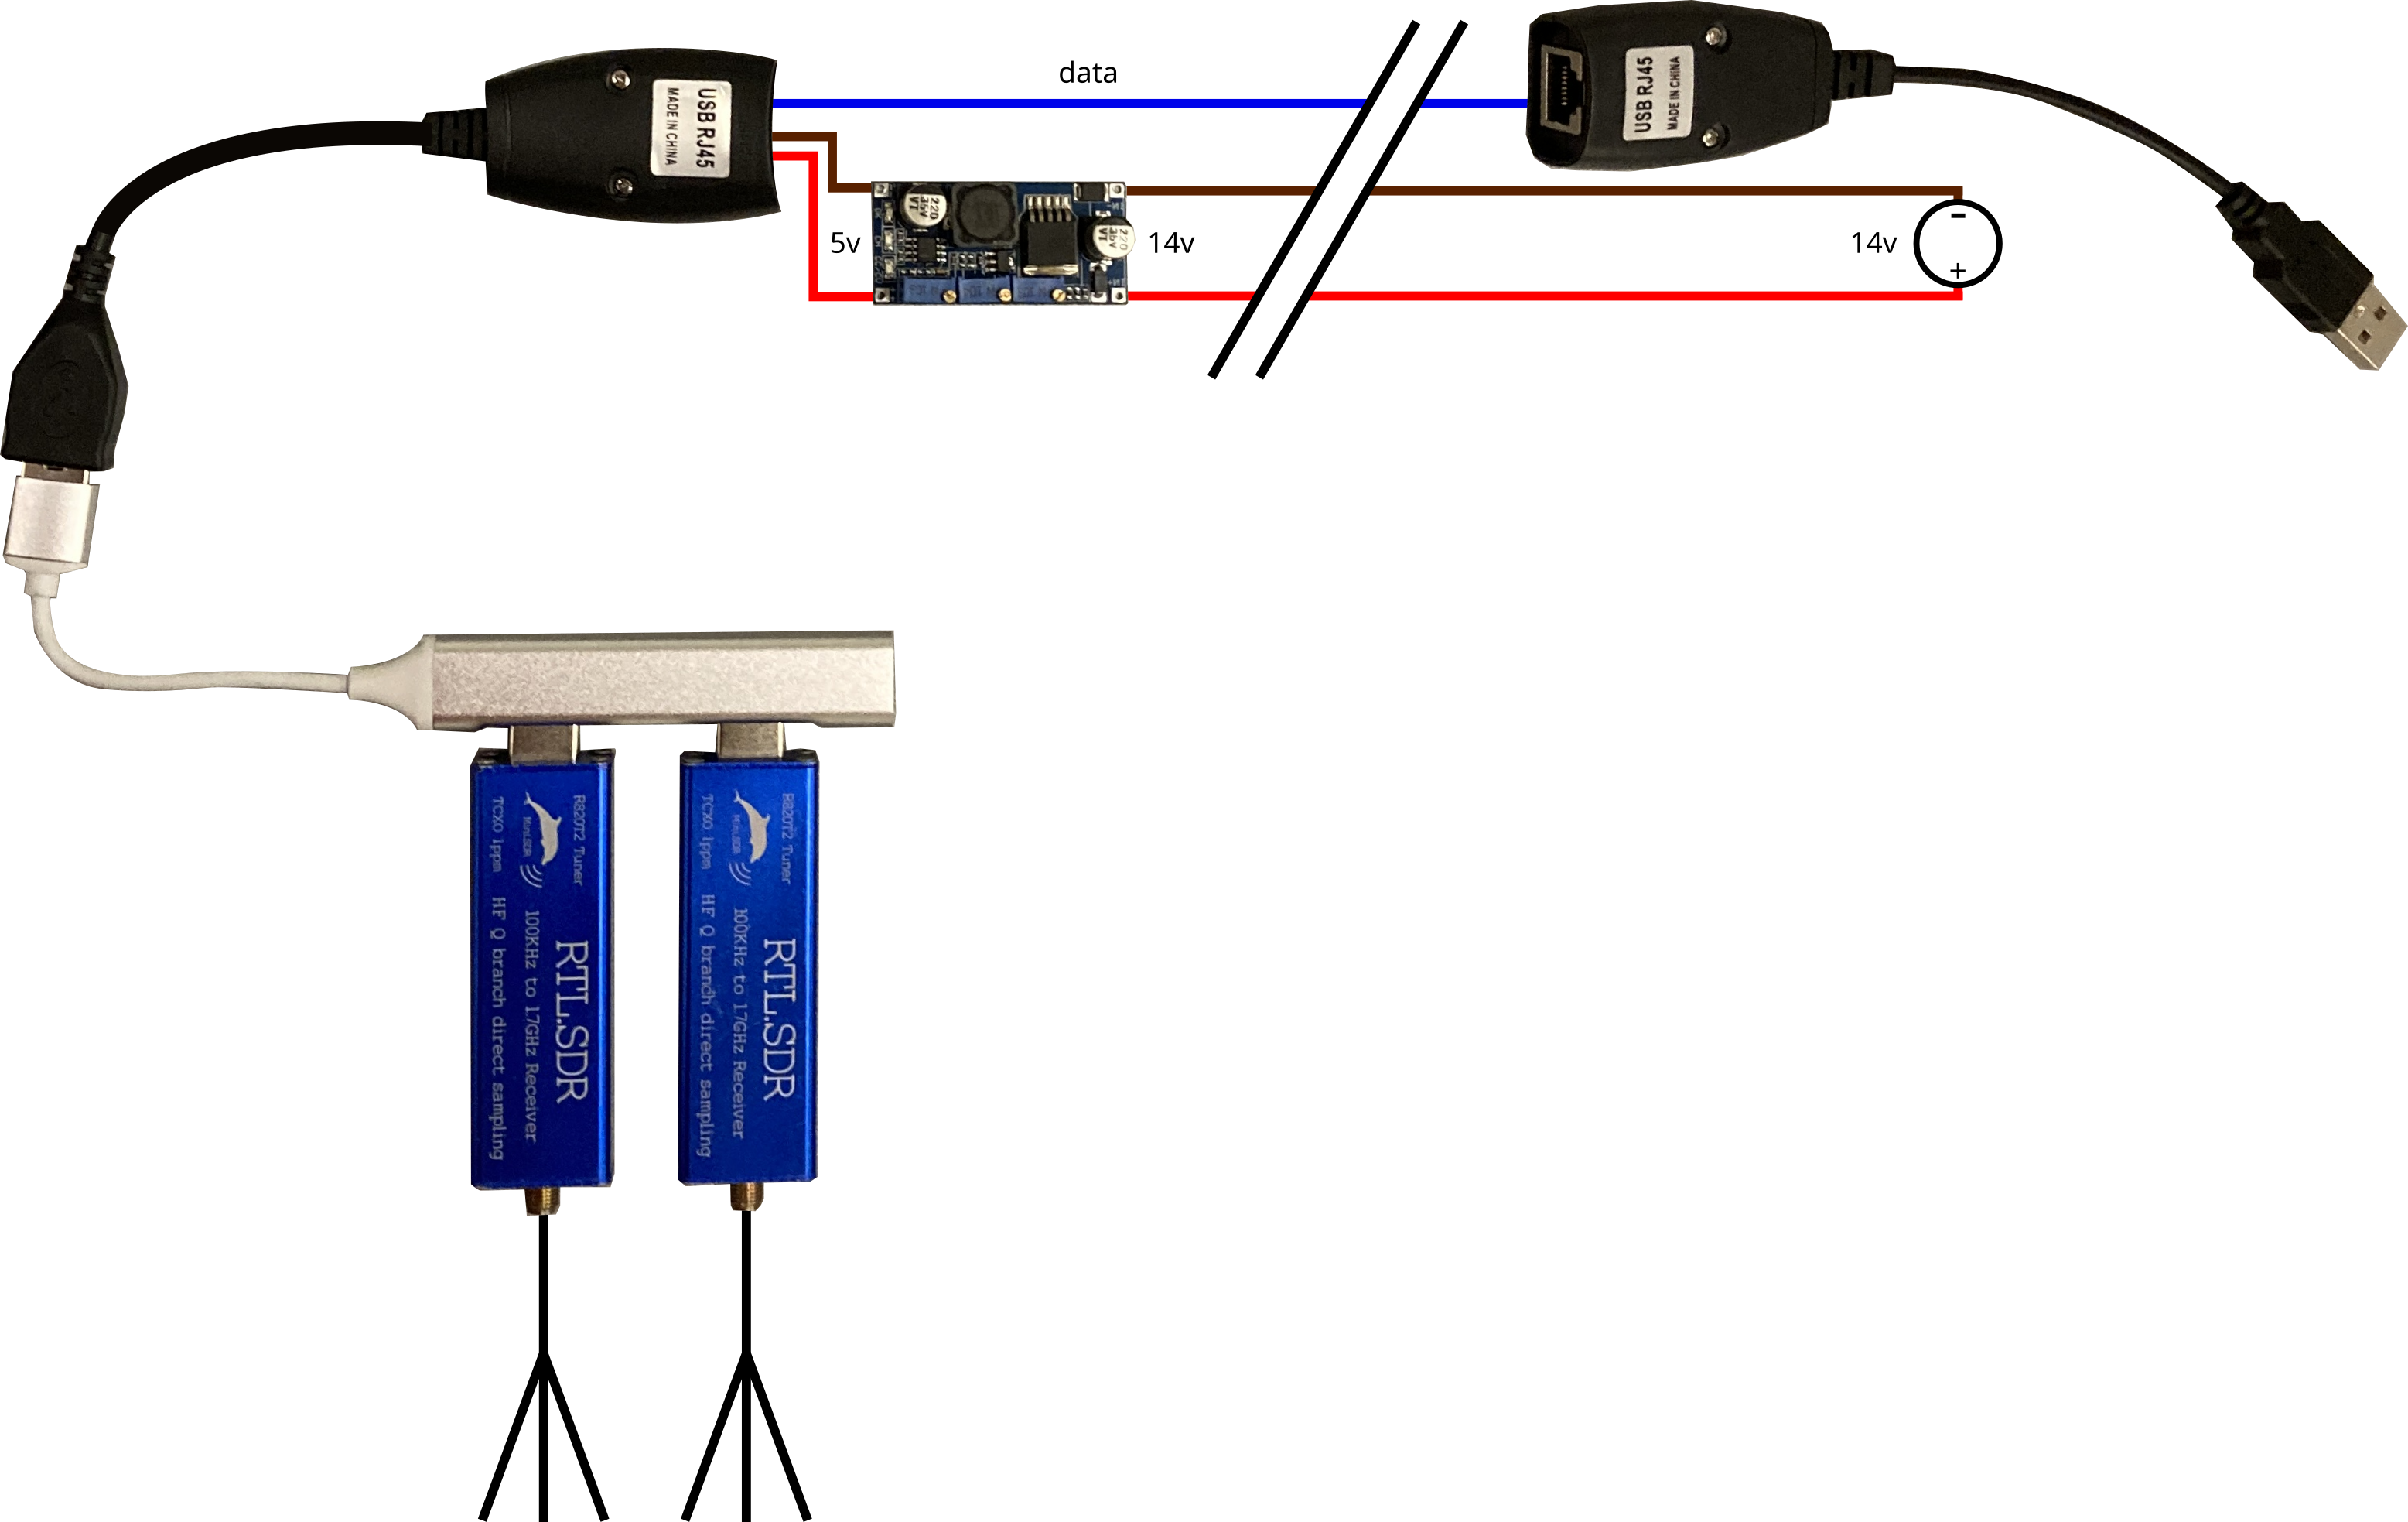
\includegraphics[width=\textwidth]{plana.png}
		\caption{Вариант архитектуры №1.}
	\end{figure}
	
	Такой вариант позволил бы уменьшить количество оборудования на крыше и его энергопотребление, упростив систему и увеличив отказоустойчивость системы по сравнению в вариантом №2. Однако, требовалось проверить, будет ли удлинитель USB предоставлять достаточную скорость передачи данных для стабильной работы системы.
	
	\pagebreak
	\subsubsection*{Вариант №2}
	\addcontentsline{toc}{subsubsection}{Вариант №2}
	
	Другим возможным вариантом представлялось подключение RTL-SDR модулей к микрокомпьютеру Raspberry Pi, который также был бы установлен на крыше, и передачу цифровых данных на управляющий компьютер для декодирования и обработки используя Ethernet.
	
	\begin{figure}[H]
		\centering
		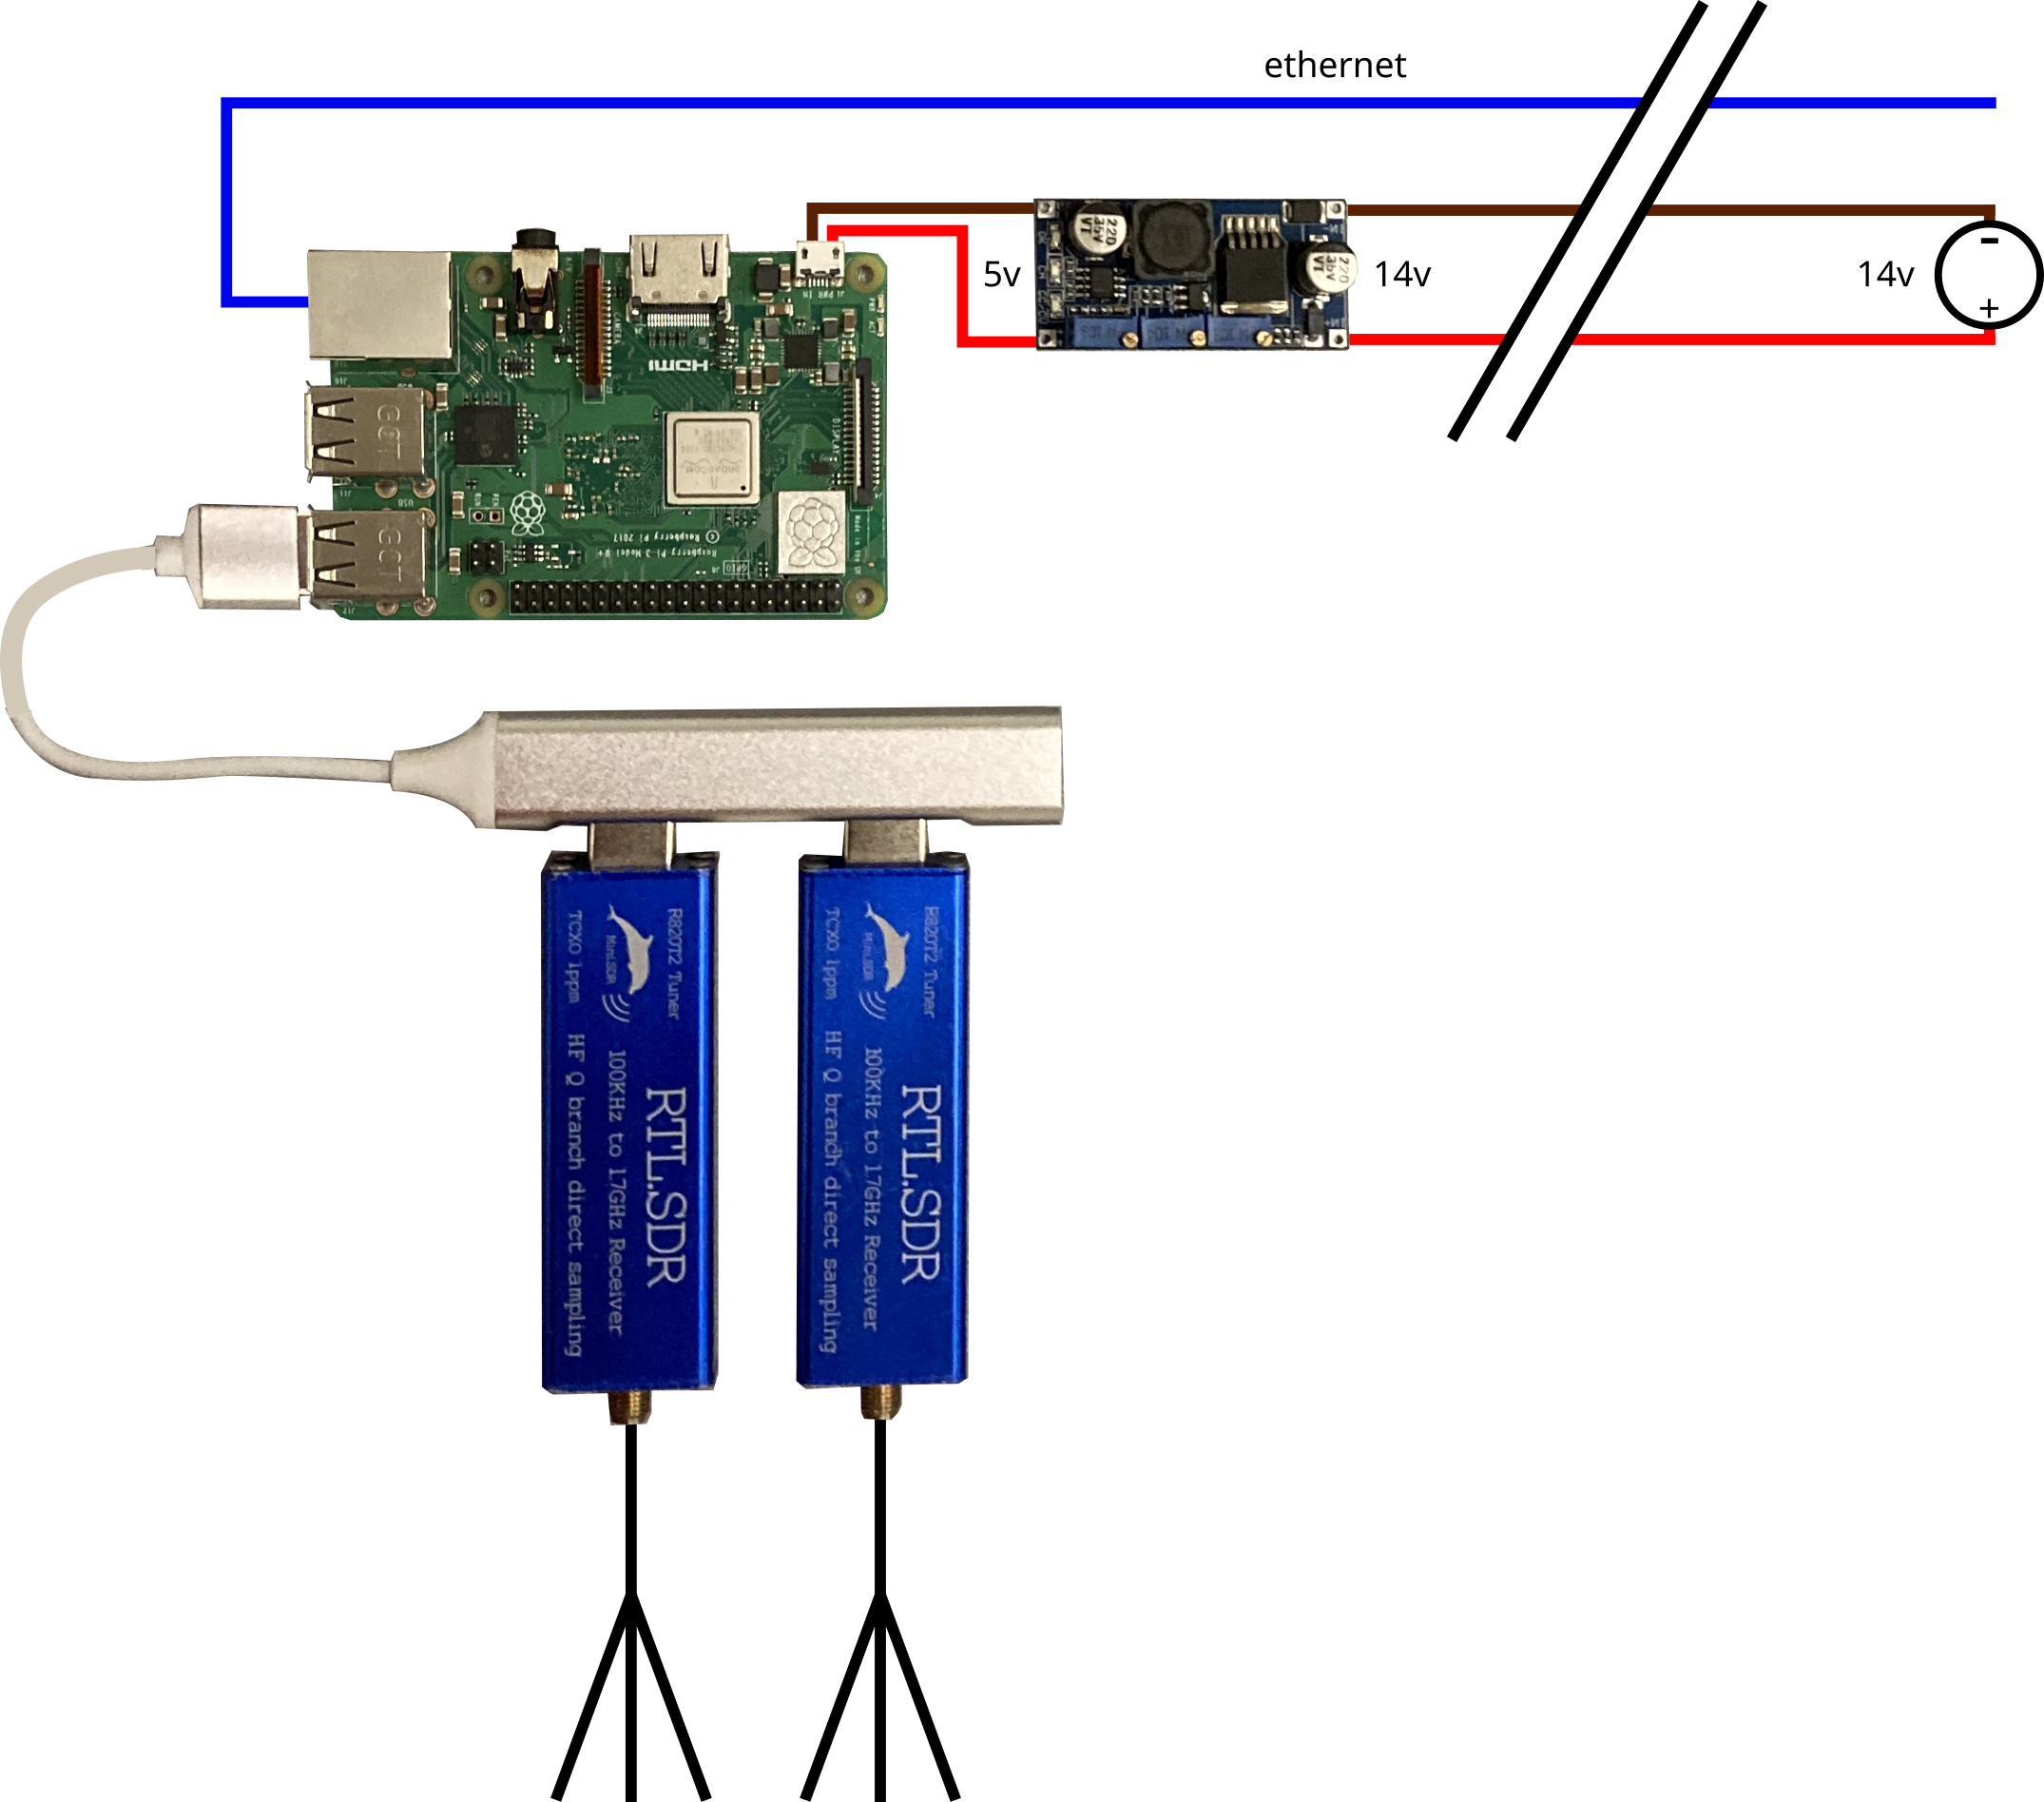
\includegraphics[width=\textwidth]{planb.png}
		\caption{Вариант архитектуры №2.}
	\end{figure}
	
	Такой вариант обеспечивал бы более высокую пропускную способность и устойчивость к магнитным помехам линии передачи данных. Однако, он требовал бы более высокой мощности питания и дополнительно потребовал бы дополнительного охлаждения, а также усложнил бы программную реализацию, отделив управляющий компьютер и радиоприёмники.
	
	\pagebreak
	\subsubsection*{Вариант №3}
	\addcontentsline{toc}{subsubsection}{Вариант №3}
	
	Последним рассмотренным вариантом являлось расположение на крыше только предусилителей, и передачи аналогового сигнала, от них по коаксиальному проводу к радиоприёмникам, расположенным в помещении.
	
	\begin{figure}[H]
		\centering
		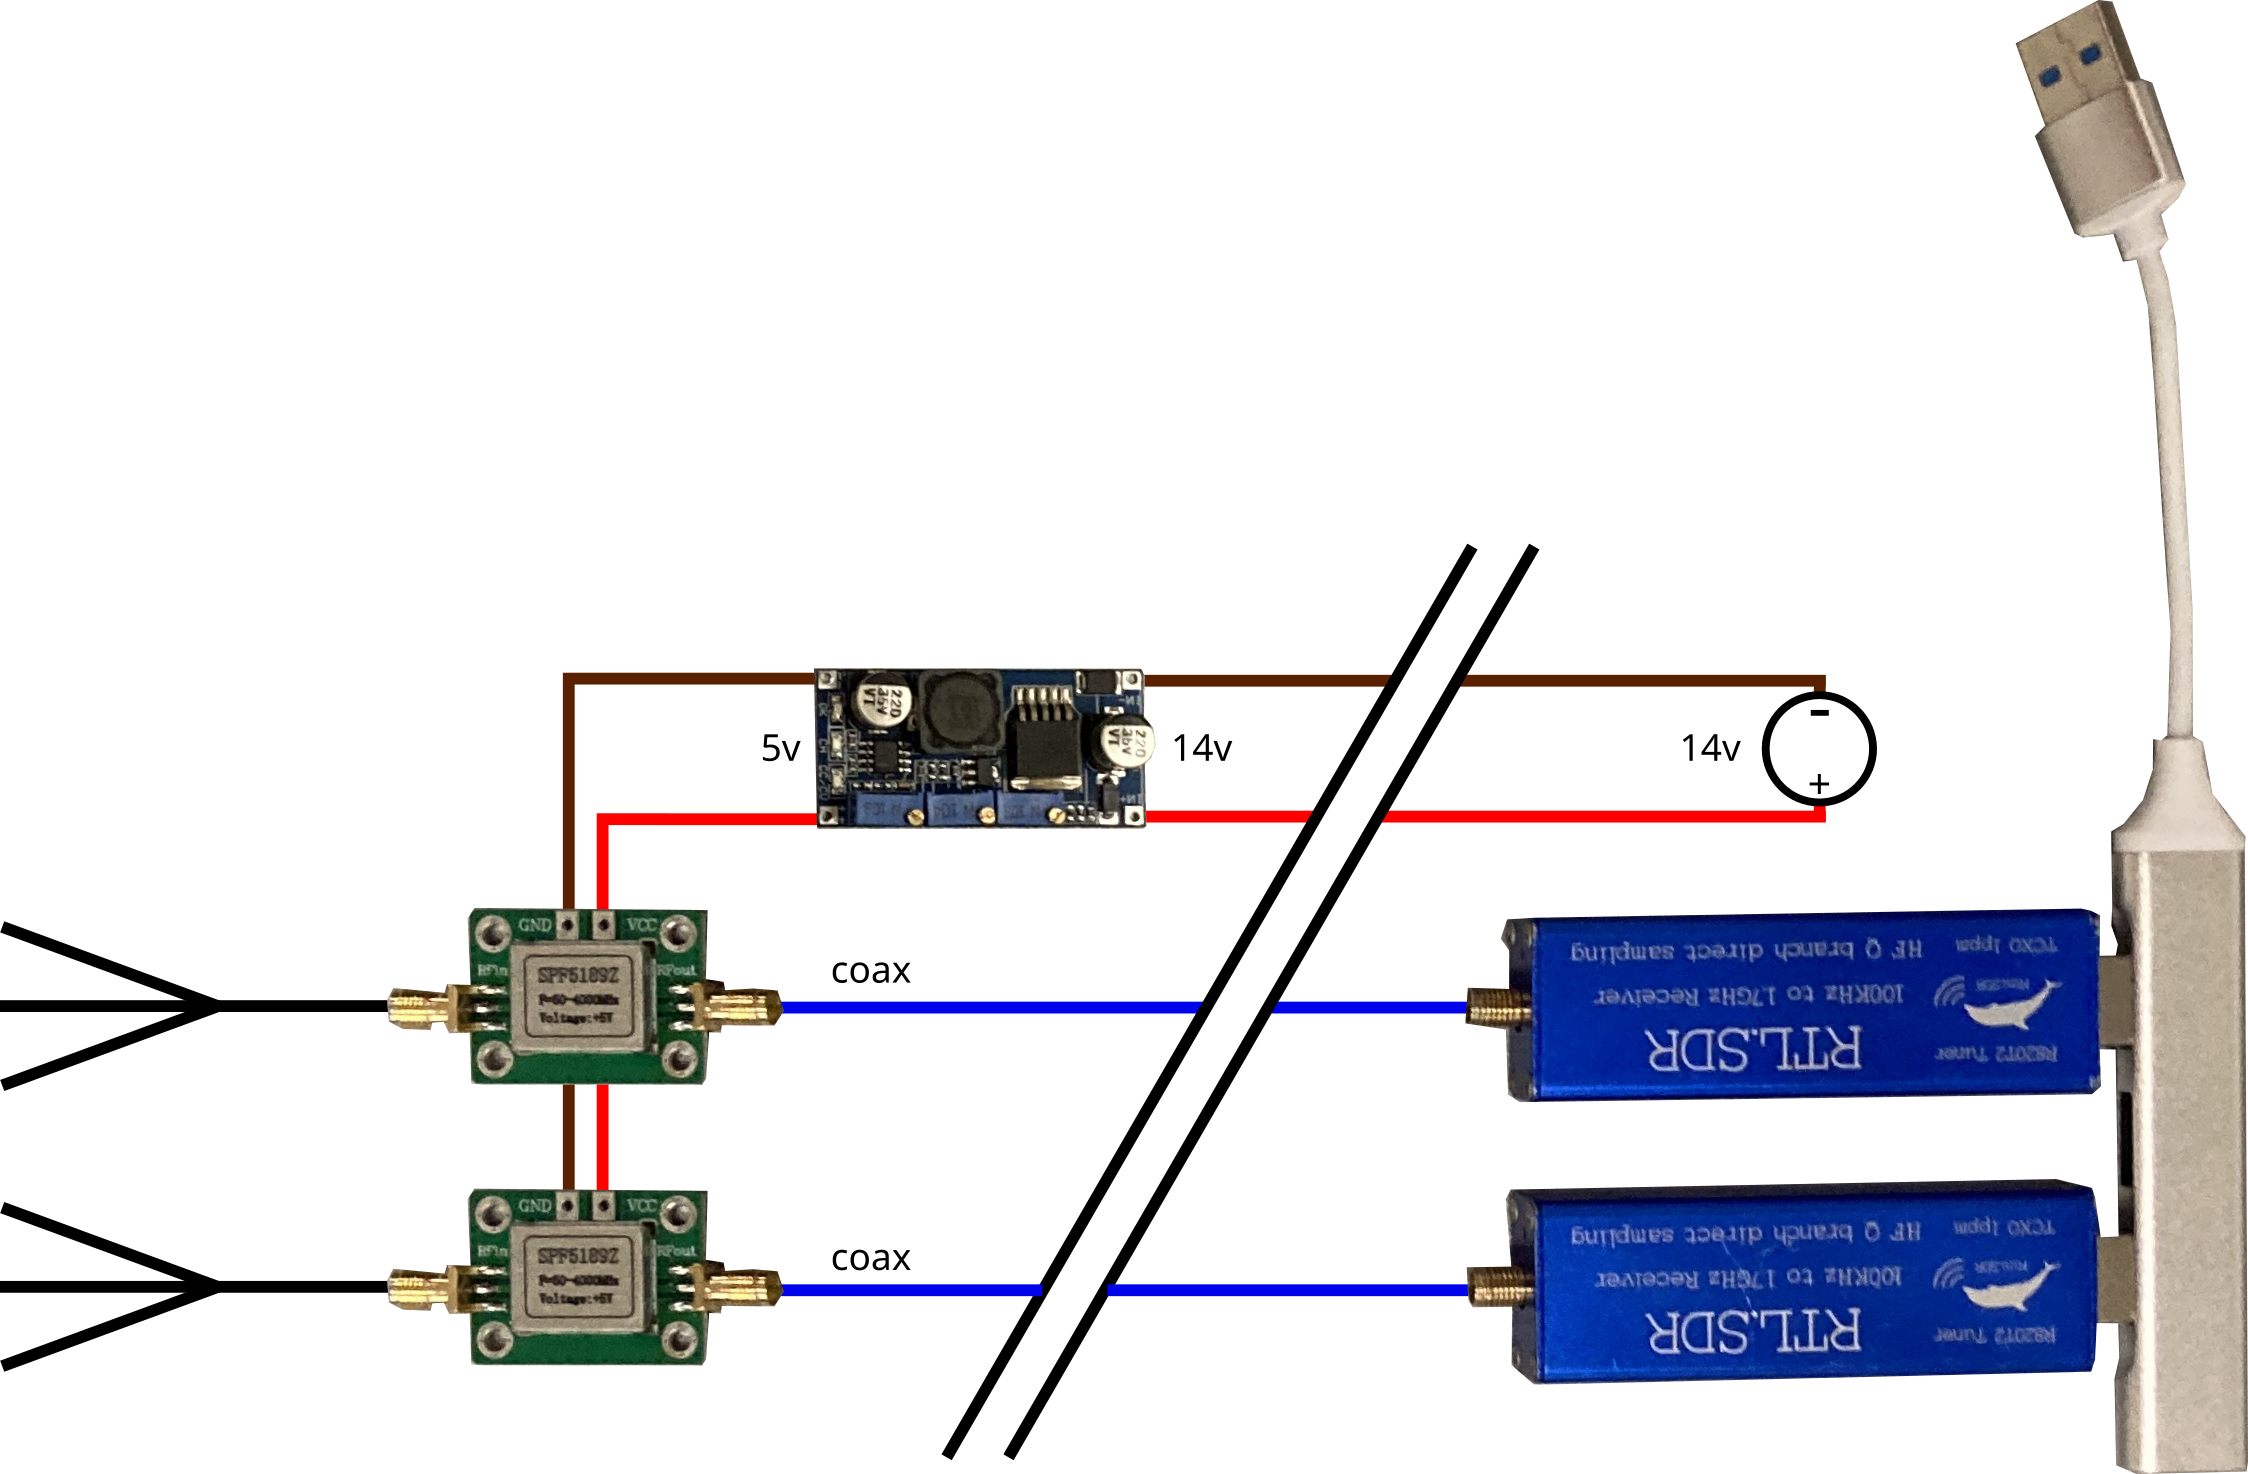
\includegraphics[width=\textwidth]{planc.png}
		\caption{Вариант архитектуры №3.}
	\end{figure}
	
	Этот вариант был бы наиболее простым в реализации, и обеспечивал бы более простую возможность ремонта и обновления системы. Однако, он был бы наиболее подвержен помехам в виду передачи аналогового а не цифрового сигнала, что дополнительно усугублялось бы возможными наводками по линии питания от инверторного понижающего регулятора.
	
	\pagebreak
	\subsection*{Реализация}
	\addcontentsline{toc}{subsection}{Реализация}
	
	Было проведено тестирование работоспособности вариантов №1 и №2 для необходимой длины линий питания и данных. Было обнаружено, что оба варианты архитектуры обеспечивают достаточное питание, однако удлинителю USB не располагают достаточной шириной канала для работы с RTL-SDR. В силу этого решено было использовать вариант архитектуры №2. Вариант №3 не был протестирован в виду того, что у нас не было коаксиального кабеля необходимой длины.
	
	В данный момент система собрана, протестирована, и готова к влагоизоляции и установке на крышу, что будет сделано как только нами будет получено соответствующее разрешение от вуза.
	
	\pagebreak
	\section*{Программная реализация}
	\addcontentsline{toc}{section}{Программная реализация}
	
	\subsection*{Автоматизация приема APT сигнала на RTL-SDR}
	\addcontentsline{toc}{subsection}{Автоматизация приема APT сигнала на RTL-SDR}
	
	Для автоматизации приема APT сигнала был реализован скрипт на языке программирования Python. \\
	
	\noindent Автоматизация заключается в следующем:
	
	\begin{itemize}
		\item \textbf{Расчет времени приема спутника}.
		\item \textbf{Запись и сохранение радио сигнала на нужной волне во время пролета спутника}.
	\end{itemize}
	
	\subsubsection*{Расчет времени приема спутника}
	\addcontentsline{toc}{subsubsection}{Расчет времени приема спутника}
	
	Что бы узнать когда мимо нас пролетает конкретный спутник, можно обратиться к уже готовым сервисам предоставляющих эту информацию и забирать её от туда. Таким сервисом стал \href{https://www.n2yo.com/?s=33591}{N2YO}. \\
	
	 N2YO - это сервис на котором можно отслежить положение спутников на орбите в реальном времени, получать о спутниках справочную информацию, а так же предсказывать время пролета спутника в конкретной точке мире, что нам и инетресно. Для обмена этой информации у сервиса N2YO есть \href{https://www.n2yo.com/api/}{API}. \\
	
	 Для получения этой информации атоматически, была написанна функция $get\_start\_record\_time$ которая обращается к API сервиса N2YO и возвращает ближайшее время пролета выброного нами спутника.
	
	\begin{minted}{Python}
CONFIG_PATH = 'config.ini'

# N2YO API -> https://www.n2yo.com/api/
def get_start_record_time(satellite_id: str, 
			  lat: str, 
			  lon: str, 
			  days: int
) -> tuple[datetime.datetime, datetime.datetime]:
    '''
    Time of passage of the specified satellite in UTC + 10h

    :param satellite_id: satellite id in n2yo
    :param lat: observer's latitide
    :param lon: observer's longitude
    :param days: number of days of prediction (max 10)
    
    :return: satellite flyby start time and satellite
    	 flyby end time
    '''
	\end{minted}
	
	\noindent Полную релизацию функции, можно найти \href{...}{тут}. \\
	
	\pagebreak
	\subsubsection*{Запиcь и сохранение радио сигнала на нужной волне во время пролета спутника}
	\addcontentsline{toc}{subsubsection}{Запись и сохранение радио сигнала на нужной волне во время пролета спутника}
	
	 \noindent Запиcь сигнала осуществлялась на RTL-SDR. Для взаимодействия Python с RTL-SDR использовалась библиотека \href{https://github.com/pothosware/SoapySDR/wiki}{SoapySDR}. \\ 
	
	\noindent SoapySDR — это набор кроссплатформенных библиотек, написанных на C++, предоставляющих унифицированный доступ к SDR-устройствам. Так же для этой библиотеки существует \href{https://github.com/pothosware/SoapySDR/wiki/PythonSupport}{оболочка на Python}, которая и была использована. \\
	
	\noindent Функция $sdr\_record$ для запиcи и сохранения радио сигнала на выбранной частоте.
	
	\begin{minted}{Python}
def sdr_record(device,
	       frequency,
	       sample_rate,
	       gain,
	       blocks_count
) -> None:
    '''
    Receiving and recording a radio signal

    :param device: sdr device object
    :param frequency: value of frequency
    :param sample_rate: value of sample rate
    :param gain: value of gain
    :param blocks_count: number of record blocks 
    '''
	\end{minted}
	
	\noindent Полную релизацию функции, можно найти \href{...}{тут}. \\
	
	\pagebreak
	\subsection*{Декодирование принятого APT сигнала спутника NOAA-19}
	\addcontentsline{toc}{subsection}{Декодирование принятого APT сигнала спутника NOAA-19}
	
	Для превращения сигнала от спутника NOAA-19 в изображение реализованн класс $NOAADecoder$.
	
	\begin{minted}{Python}
class NOAADecoder:
    def __init__(self,
                 black_point: int,
                 white_point: int,
                 components: Optional(List[str]),
                ) -> None:
        '''
        Class for decode NOAA APT data

        :param black_point: dynamic range lower bound, 
        		percent
        :param white_point: dynamic range upper bound, 
        		percent
        :param components: portions of the image to 
        		preserve/filter
        '''
	\end{minted}
	
	\noindent Полную релизацию функции, можно найти \href{...}{тут}. \\
	
	\noindent Декодирование сигнала в изображение происходит следующим образом:
	
	\begin{itemize}
		\item \textbf{Передискретизация до частоты 20800 Гц}.
		\item \textbf{Преобразование в аналитический сигнал (\href{https://en.wikipedia.org/wiki/Hilbert_transform}{Преобразование Гилберта})}.
		\item \textbf{Нормирование значний сигнала от 0 до 255}.
		\item \textbf{Нахождение положения кадров синхронизации сигнала APT}.
		\item \textbf{Выбор сектора для формирования изображения}.
	\end{itemize}
	
\end{document}		